\documentclass{article}
\usepackage[utf8]{inputenc}
\usepackage[english, swedish]{babel}

\usepackage{cite}
\usepackage{caption}
\usepackage{graphicx}
\usepackage{float}
\usepackage{textcomp}
\usepackage{listings}
\usepackage{color}
 
\definecolor{codegreen}{rgb}{0,0.6,0}
\definecolor{codegray}{rgb}{0.5,0.5,0.5}
\definecolor{codepurple}{rgb}{0.58,0,0.82}
\definecolor{backcolour}{rgb}{0.95,0.95,0.92}
 
\lstdefinestyle{mystyle}{
    backgroundcolor=\color{backcolour},   
    commentstyle=\color{codegreen},
    keywordstyle=\color{magenta},
    numberstyle=\tiny\color{codegray},
    stringstyle=\color{codepurple},
    basicstyle=\footnotesize,
    breakatwhitespace=false,         
    breaklines=true,                 
    captionpos=b,                    
    keepspaces=true,                 
    numbers=left,                    
    numbersep=5pt,                  
    showspaces=false,                
    showstringspaces=false,
    showtabs=false,                  
    tabsize=2
}

\lstset{style=mystyle}

\usepackage[yyyymmdd]{datetime}
\renewcommand{\dateseparator}{-}

\usepackage{graphicx}
\graphicspath{ {images/} }

%For headers & footers
\usepackage{fancyhdr}
\pagestyle{fancy}
\lhead{
\includegraphics[scale=0.2]{Logo}}
\chead{Kartrobot}
\rhead{\today}

\lfoot{Konstruktion med mikrodatorer}
\rfoot{Grupp 3}

\usepackage{titlesec}

\setcounter{secnumdepth}{4}

\titleformat{\paragraph}
{\normalfont\normalsize\bfseries}{\theparagraph}{1em}{}
\titlespacing*{\paragraph}
{0pt}{3.25ex plus 1ex minus .2ex}{1.5ex plus .2ex}

\renewcommand{\headrulewidth}{0.4pt}
\renewcommand{\footrulewidth}{0.4pt}


\title{Teknisk dokumentation för kartrobot}
\author{Patrik Sletmo}
\date{\today}

\selectlanguage{swedish}

\begin{document}

\thispagestyle{empty}

{
\sffamily
\centering
\large


{\huge 
Teknisk dokumentation för kartrobot
}

{\large
Patrik Sletmo
}

{\large
Version 1.0
}

\vspace{3.5cm}

Status
\begin{table}[H]
\centering
\begin{tabular}{ | c | c | c | }
\hline
STATUS & Patrik Sletmo & 2016-12-DD \\
\hline
\end{tabular}
\end{table}
}
\clearpage

\vspace*{\fill}
{
\sffamily
\centering
\large


{\huge
Projektidentitet
}

{\large
Grupp 3, 16/HT, KarToffel \\ Linköpings tekniska högskola, ISY
}

\vspace{0.5cm}

\begin{table}[H]
\centering
\begin{tabular}{ | c | c | c | c |}
\hline
Namn & Ansvar & Telefon & E-post \\
\hline
Patrik Sletmo & Projektledare & 070 783 57 61 & patsl736@student.liu.se \\
\hline
Rebecca Lindblom & Utvecklare & 073 436 40 79 & rebli156@student.liu.se \\
\hline
Matildha Sjöstedt & Utvecklare & 070 515 84 11 & matsj696@student.liu.se \\
\hline
Sebastian Callh & Utvecklare & 073 820 46 64 & sebca553@student.liu.se \\
\hline
Anton Dalgren & Utvecklare & 076 836 51 56 & antda685@student.liu.se \\
\hline
Matilda Dahlström & Utvecklare & 070 636 33 52 & matda715@student.liu.se \\
\hline
\end{tabular}
\end{table}
}

\begin{center}
\textbf{Hemsida}: https://github.com/SebastianCallh/kartoffel-tsea29
\end{center}

\begin{center}
\textbf{Kund}: Mattias Krysander, 013 - 28 2198 , matkr@isy.liu.se
\end{center}

\begin{center}
\textbf{Kursansvarig}: Tomas Svensson, 3B 528, +46 (0)13 28 1368, tomas.svensson@liu.se \\
\textbf{Handledare}: Anders Nilsson, 3B 512, +46 (0)13 28 2635, anders.p.nilsson@liu.se
\end{center}
\vspace*{\fill}
\clearpage

\renewcommand*\contentsname{Innehållsförteckning}
\tableofcontents
\clearpage


{
\sffamily
\centering
\large


{\huge 
Dokumenthistorik \\
}
\begin{table}[H]
\centering
\begin{tabular}{ | c | c | c | c | c |} 
\hline
\textbf{Version} & \textbf{Datum} & \textbf{Utförda ändringar} & \textbf{Utförd av } & \textbf{Granskad} \\
\hline
VERSION & 2016-12-DD & Första version & Grupp 3 & Patrik Sletmo \\
\hline

\end{tabular}
\end{table}
}

\clearpage
\section{Inledning}

\subsection{Bakgrund}
Som en del av utbildningen till civilingenjör i datateknik på Tekniska Högskolan vid Linköpings Universitet har vår projektgrupp i kursen Konstruktion med mikrodatorer (TSEA29) arbetat mot beställaren Mattias Krysander för att tillverka en robot vars syfte är att kartlägga en sluten bana. Den färdiga produkten tävlar mot andra gruppers robotar och redovisas i samband med kursens avslutande.

\subsection{Syfte}
Det här dokumentet skall ge en ingående beskrivning av kartrobot-systemet från ett tekniskt perspektiv. Dokumentet ska fungera som konstruktionsunderlag för någon som vill bygga en kopia av den robot som beskrivs. Det ska från instruktioner i dokumentet även vara möjligt att underhålla och felsöka både mjuk- och hårdvaran i systemet.

\clearpage
\section{Produkten}
%En bild på produkten och en beskrivning av hur den fungerar. Beskriv vad den används till.

Systemet består av en fyrhjulig robot samt en mjukvaruklient som kommunicerar med varandra via Bluetooth. Systemets syfte är att roboten ska kunna kartlägga sin omgivning helt autonomnt och förmedla kartläggningen till mjukvaruklienten. För att göra det så är den utrustad med diverse IR-sensorer, en lasersensor och ett gyroskop för att kunna navigera och mäta avstånd. Se figur~\ref{fig:robot_bild} för en bild på konstruktionen.

\begin{figure}[H]
\centering

\includegraphics[scale=0.45]{Logo}
\caption{En bild på roboten.}
\label{fig:robot_bild}
\end{figure}

Mjukvaruklienten är som nämnt ansluten via Bluetooth, vilket låter den rendera kartläggningen i realtid. Den har även ett gränssnitt för att kunna fjärrstyra roboten. Se figur~\ref{fig:klient_bild} för en bild på mjukvaruklientens gränssnitt.

\begin{figure}[H]
\centering

\includegraphics[scale=0.45]{Logo}
\caption{En bild på mjukvaruklienten.}
\label{fig:klient_bild}
\end{figure}

\clearpage
\section{Teori}
% Beskrivning av regleralgoritmer mm.
Den övergripande strategin för att kratlägga rummet är att alltid färdas längst väggen på höger sida och på så sätt kartlägga rummets ytterväggar. För det krävs en regleringsalgoritm för att följa väggen och logik för navigering samt kartläggning.

\subsection{Navigering}
~\label{sec:navigering}
Navigeringslogiken implementeras som en tillståndsmaskin vars transitioner styrs av indata från robotens sensorer. Den antar att omgivningen följer banspecifikationen i bilaga~\ref{sec:banspec}.

Efter en kort uppvärmningsperiod för att hinna läsa in alla sensorer så börjar roboten följa väggen på sin högra sida och håller ett lämplig avstånd till den med hjälp av PD-reglering (se ~\ref{sec:reglering}). Om roboten upptäcker att väggen på höger sida tar slut så innebär det att väggen har svängt av bort från roboten och att den behöver göra en yttersväng till höger för att följa efter. Skulle roboten upptäcka en vägg framför sig betyder det istället att rummet svängt av till vänster, och att roboten behöver göra in innersväng åt vänster. Ett flödesdiagram över robotens navigeringstillstånd kan ses i figur~\ref{fig:navigator_flowchart}.

\begin{figure}[H]
\centering
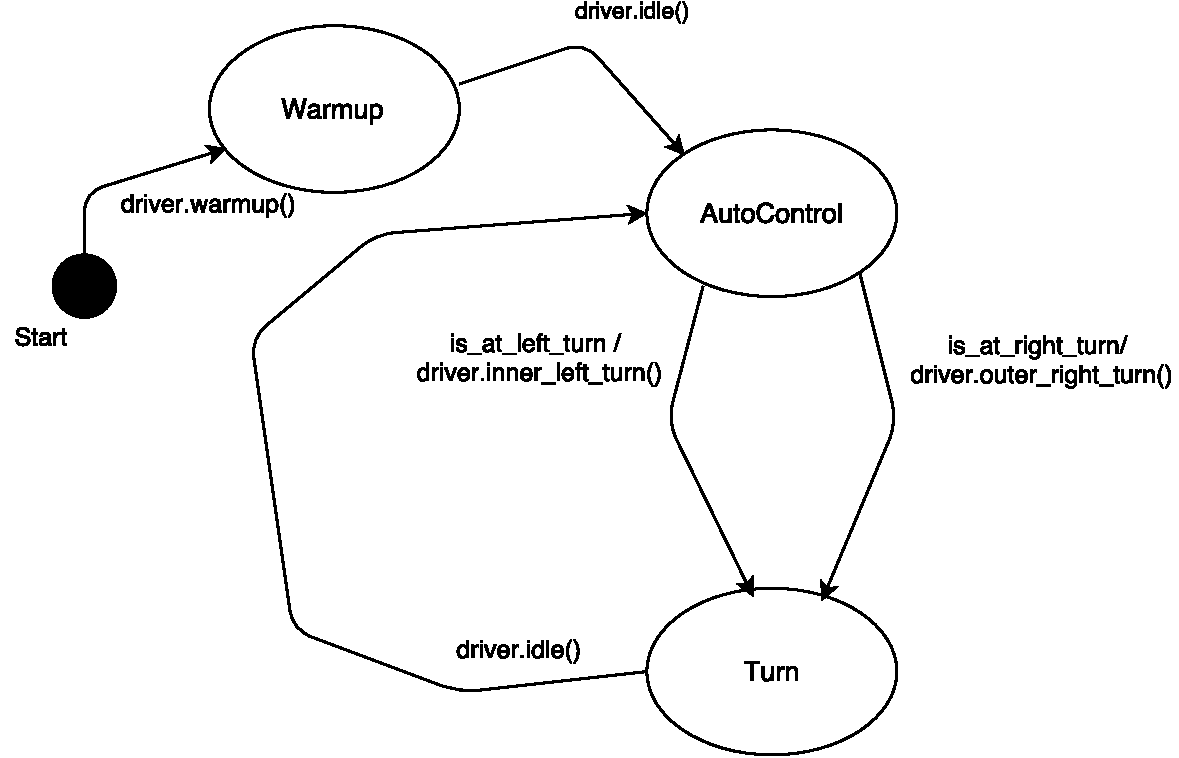
\includegraphics[scale=0.4]{navigator_flowchart}
\caption{Ett flödesdiagram på navigatorns tillstånd.}
\label{fig:navigator_flowchart}
\end{figure}

\subsection{Kartläggning}

\subsection{Reglering}
 ~\label{sec:reglering}
 
 \subsection{PMM}
~\label{sec:PWM}

\subsection{Kommunikation}
Systemet byggs upp av ett antal separata moduler som behöver samarbeta för att utföra robotens funktion då dess unika funktioner är alldeles för specifika. Kommunikationen som möjliggör detta samarbete sker både via Bluetooth och I2C beroende på modulernas placering i systemet. Då det kan bli förvirrande att hantera dataflödet på två olika protokoll ligger det ett abstraktionslager som kallas EventBus ovanpå dessa överföringsmedier. Detta abstraktionslager samt de underliggande implementationerna beskrivs mer ingående i följande delavsnitt. 

\subsubsection{EventBus}
För att underlätta programmering av logikenheten använder sig systemet av en distribuerad eventbuss kallad EventBus som tillhandahåller funktioner för att skicka data till en annan enhet på bussen och för att lyssna på mottagna meddelanden. Eventbussen är delad mellan sensorenheten, styrenheten, huvudenheten samt mjukvaruklienten men eftersom bussen saknar funktionalitet för att delegera data vidare till andra enheter kan data inte skickas direkt från t.ex. sensorenheten till styrenheten, se figur~\ref{fig:eventbus_structure}. Eventbussen saknar fysiskt representation i den mening som t.ex. I2C-bussen har utan är bara en abstraktion som med hjälp av I2C-bussen och Bluetooth-anslutningen realiserar dess distribuerade funktion.

\begin{figure}[H]
\centering
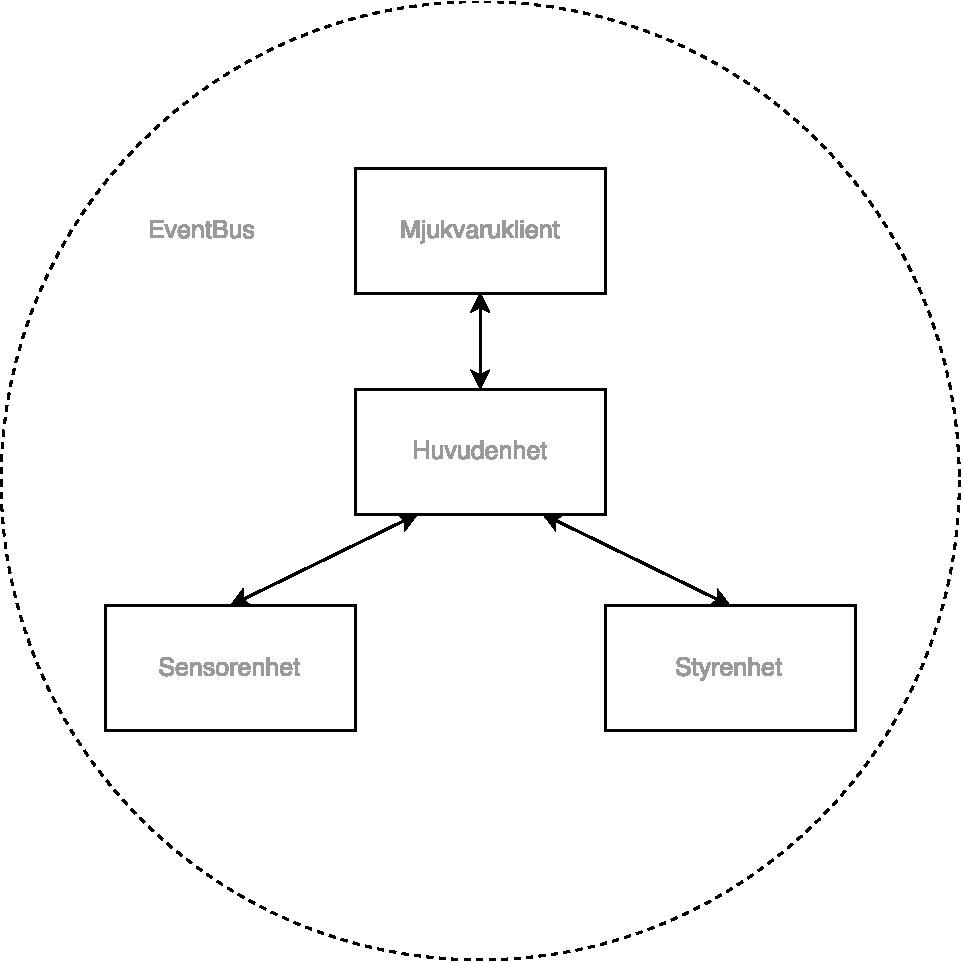
\includegraphics[scale=0.45]{EventBus}
\caption{Översikt över eventbussens möjliga kommunikationsriktningar}
\label{fig:eventbus_structure}
\end{figure}
\ \\
\newline
Tanken med eventbussen är att programmeraren ska slippa tänka på att ett funktionsanrop exekveras på en annan enhet eller varifrån data kommer, så länge det läggs åtanke på att funktionerna exekveras asynkront. All mottagen data behöver manuellt behandlas i ett periodiskt funktionsanrop innan de ``lyssnande'' funktionsanropen körs. För att få en tydligare och mer deterministisk körning av huvudenhetens program läses all mottagen data in i början av varje upprepning av huvudloopen. Data ut från huvudenheten skickas till skillnad från inläsningen direkt när anropet sker för att säkerställa att data kommer fram i andra änden så tidigt som möjligt.

\subsubsection{Bluetooth}
TODO:TEXT OM BLUETOOTH. UPPDATERA SÅ DEN REFLEKTERAR VÅR IMPLEMENTATION. UPPDATERA BILD

\begin{figure}[H]
\centering

\includegraphics[scale=0.45]{Logo}
\caption{Flödesschema över Bluetooth-kommunikationen i huvudenheten.}
\label{fig:Kommunikation_huvudenhet_v2}
\end{figure}
\ \\

Bluetooth kommunikationen i huvudenheten fungerar på så vis att huvudprogrammet kommunicerar via det allmänna gränssnittet EventBus till en bluetooth-server. Servern körs i en separat process än huvudprogrammet på huvudenheten och kommer ständigt kolla om det finns ny data att ta emot respektive ny data att skicka (se figur ~\ref{fig:Kommunikation_huvudenhet_v2}), tills den får ett omstart kommando. Kommandon till huvudenheten samlas i en inkö som EventBus hämtar ifrån, på samma sätt samlas kommandon som skickas till EventBus - med destination bluetoothklienten - i en utkö där servern hämtar ifrån. Dessa in- och utköer gör det även möjligt för processen som servern ligger i och huvudprocossen där huvudprogrammet och EventBus ligger i att kommunicera. 

\subsubsection{I2C}
För att kunna kommunicera med olika moduler och sensorer på själva roboten används en I2C-buss som delas mellan huvudenheten, sensorenheten, styrenheten, laser-sensorn, gyroskopet samt accelerometern där huvudenheten agerar master och alla andra enheter slavar. Eftersom kraven som ställs på kommunikationen mellan modulerna förutsätter att data kan skickas i form av anrop räcker inte I2C-bussens protokoll till utan skrivningen och inläsningen till/från adresser behöver utökas med funktionalitet för att skicka faktiska datapaket. Det påliggande protokollet implementerar köer av paket för båda datariktningarna på AVR:erna som pollas och fylls på från huvudenheten. Varje paket innehåller ett antal bytes för dess data där den första byten innehåller paketets id. Eftersom I2C endast tillåter läsning eller skrivning av en enda byte innehåller varje paket on-the-wire också en inledande byte som specificerar dess längd, vilket ger en maxlängd av 255 bytes. När ett paket lästs in läggs det i en intern kö som hanteras av den modulspecifika koden, se figur~\ref{fig:flodesschema_i2c}.

\begin{figure}[H]
\centering
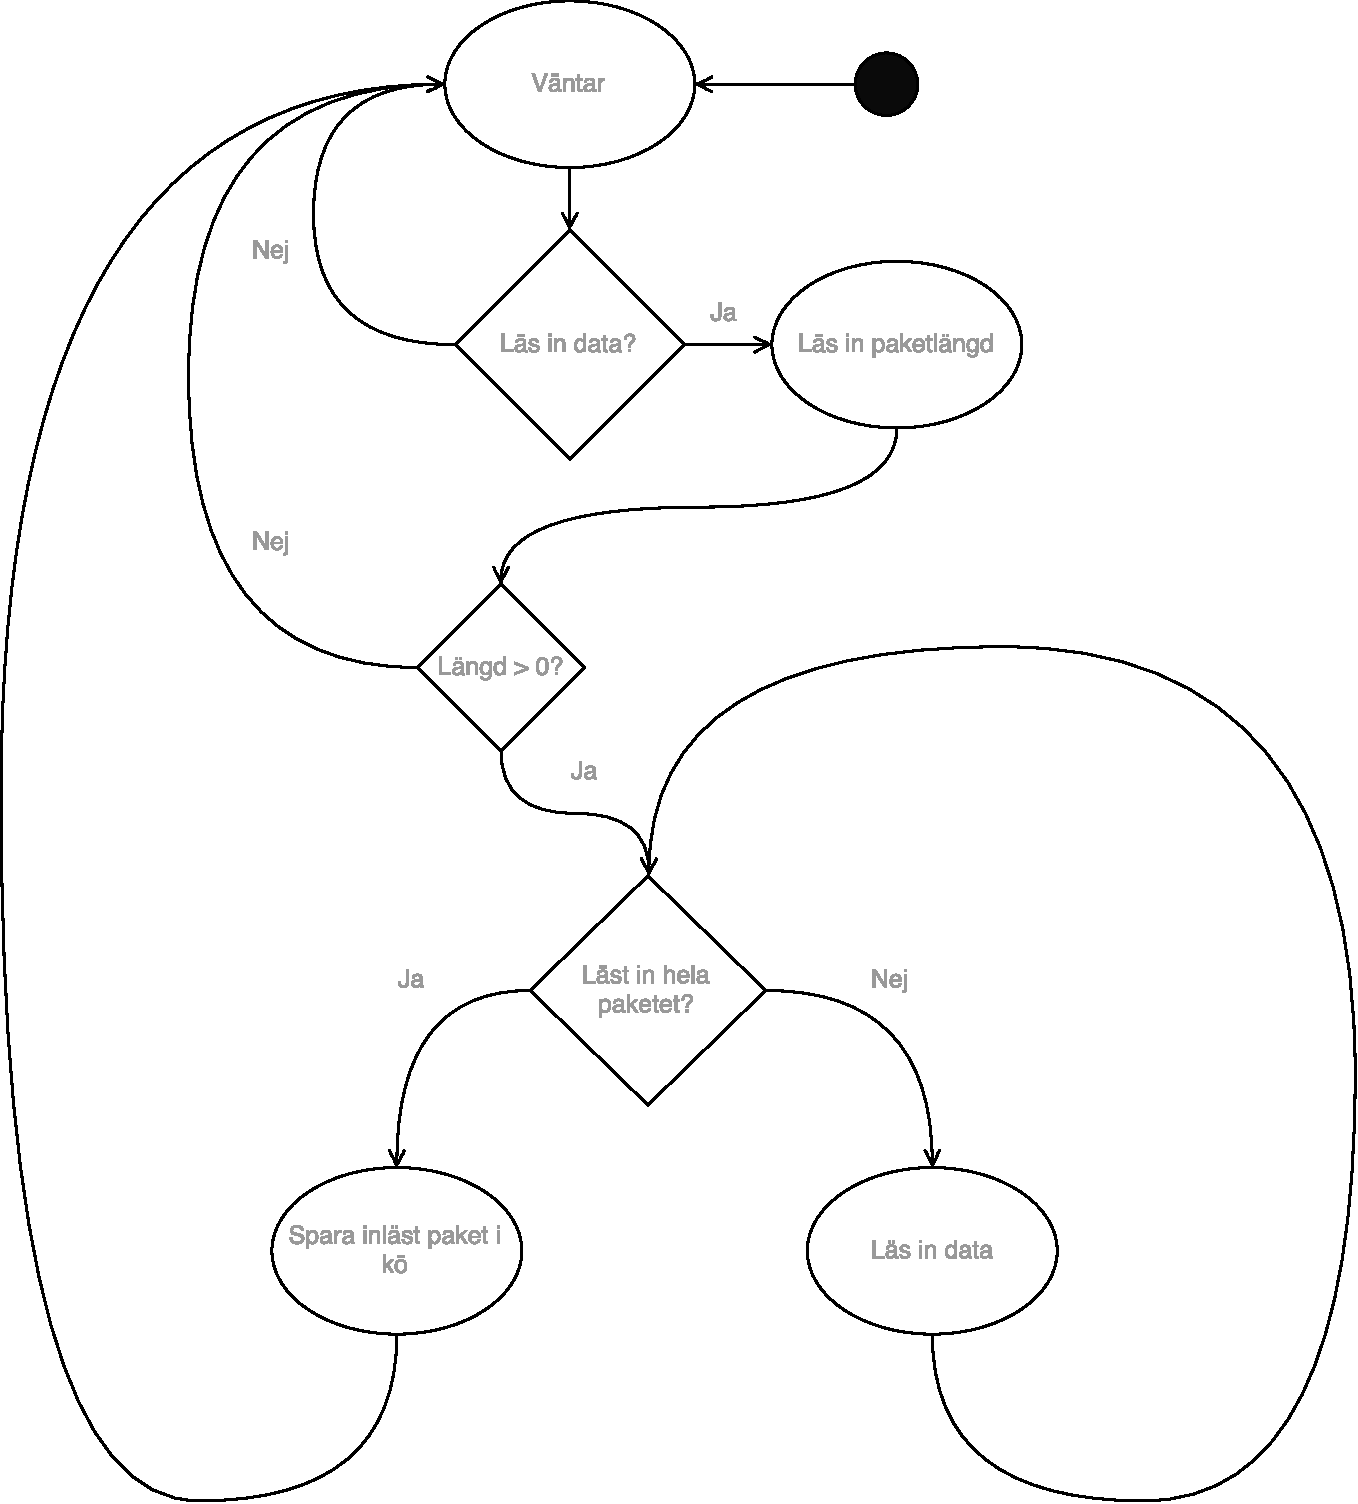
\includegraphics[scale=0.45]{Flodesschema_i2c}
\caption{Flödesschema över I2C-kommunikationen}
\label{fig:flodesschema_i2c}
\end{figure}
\ \\
\newline
Alla inkopplade enheter på I2C-bussen använder sig inte av det protokoll som beskrivs ovan utan fungerar på det vanliga sättet genom läsning och skrivning till adresser. Dessa enheter är laser-sensorn, gyroskopet samt accelerometern och adresseras direkt från huvudenheten istället för att passera via sensorenheten som alla andra sensorer till följd av begränsningar som följer från single-master implementationen. Läsning från dessa sensorer sker periodvist i huvudenhetens programloop och sparas undan så att olika delar av programmet kan komma åt det senaste datat utan att behöva läsa multipla gånger.

\clearpage
\section{Systemet}
% Ett översiktligt blockschema och en beskrivning av hela systemet.
TODO:Text om systemet i helhet

\begin{figure}[H]
\centering
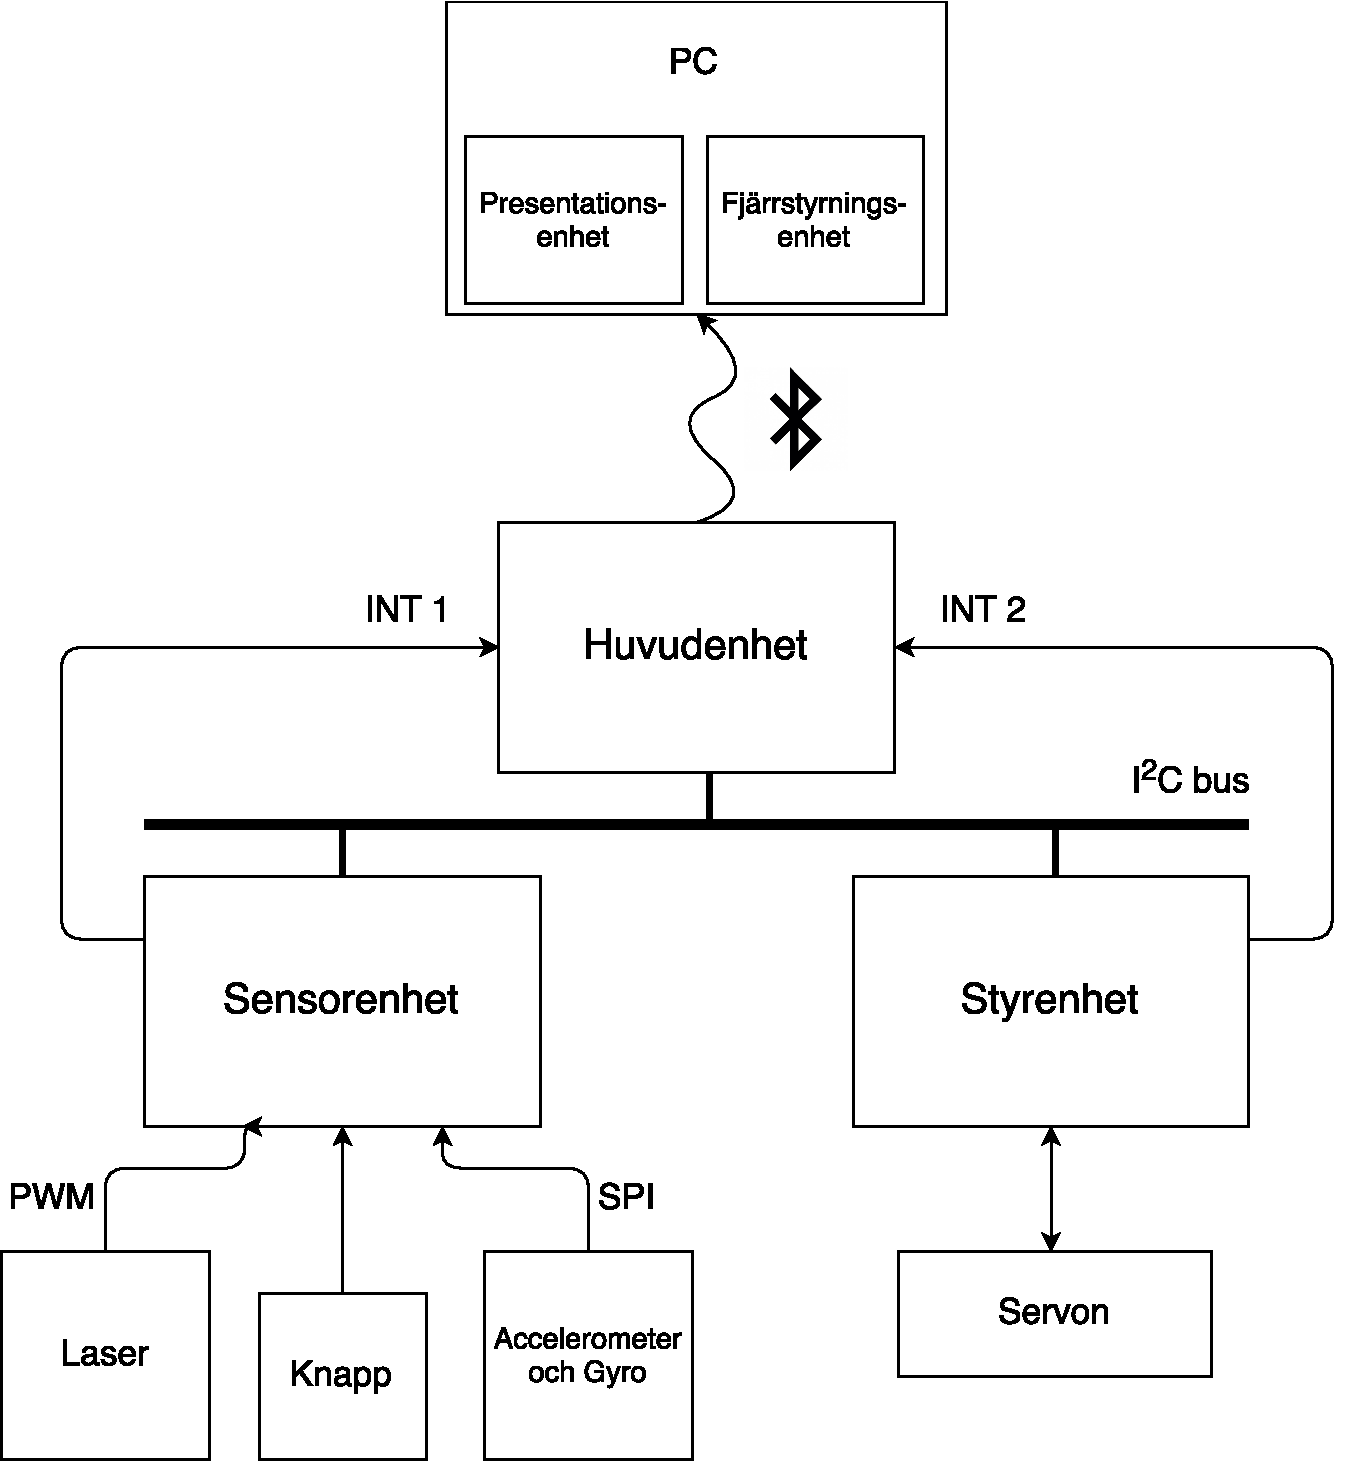
\includegraphics[scale=0.4]{oversikt_systemet}
\caption{En bild på systemet övergripande konstruktion.}
\label{fig:oversikt_systemet}
\end{figure}

\subsection{Felsökning av mjukvara}
Systemet är redan från början av projektet designat för att vara lätt att felsöka. Det finns enkla gränssnitt både in och ut från robotens alla processorer som gör att data kan manipuleras och inspekteras utan att behöva pausa programmet eller spara undan data i filer.

\subsubsection{Felsökning på AVR}
Eftersom AVR:erna i sitt grundutförande inte kan ge någon avancerad utdata finns möjligheten att på roboten koppla varje AVR direkt till en dators USB-port med hjälp av en seriell anslutningskabel. Genom att öppna seriellporten i t.ex. Putty (Windows) eller screen (UNIX) kan data skickas fram och tillbaka mellan datorn och mikroprocessorn, se listing~\ref{lst:avr_debug_screen}. I den nuvarande konfigurationen stöds bara möjligheten att skicka data från roboten till datorn men gränssnittet stödjer även den motsatta datariktningen. Implementationen bygger på att ersätta stdout-strömmen så utskrift till dator kan göras med det bekanta gränssnitt som definieras i stdio.h, se listing~\ref{lst:avr_debug_example} för ett komplett exempel.
\newline
\begin{lstlisting}[language=sh, label={lst:avr_debug_screen}, caption={Anslutning via screen}]
$ screen /dev/tty.usbserial
\end{lstlisting}

\begin{lstlisting}[language=C, label={lst:avr_debug_example}, caption=Exempel av utskrift]
#include "common/debug.h"

int measuredValue = 42;
printf("Measured value: %d\n", measuredValue);
\end{lstlisting}

\subsubsection{Felsökning på Huvudenhet}
Huvudenheten består av en Raspberry PI och kör kod skriven i Python, vilket gör att dess felsökningsmöjligheter är nästintill så bra som det går. Enklast är att ansluta sig till huvudenheten med en SSH-uppkoppling över Eduroam men det går även att koppla in tangentbord, mus och skärm direkt till roboten om så önskas. För att ansluta till enheten via SSH så loggar man in med användaren ``pi'' på den IP-adress som visas på robotens display och anger användarens lösenord. Notera att displayens innehåll uppdateras varje minut-omslag och det kan dröja ett par minuter innan roboten kopplar upp sig mot nätverket första gången.

\subsection{Felsökning av hårdvara}
På grund av varierande spänningsnivåer så inträffar det ibland fel i hårdvaran där mjukvaran har svårigheter att korrigera för felet på egen hand. De vanligaste felen och dess lösningar beskrivs i detta avsnitt.

\subsubsection{Låg batterispänning}
I stort sätt alla fel som uppkommer i hårdvaran beror på en för låg batterispänning. Det finns inget sätt att kontrollera robotens batterispänning från mjukvaruklienten eller huvudenhetens terminal utan batteriet måste avmonteras från roboten för att därefter testas med en multimeter. Lättast sättet att upptäcka att batteriet har för låg spänning är genom att observera robotens beteende. Vanliga symptom är:

\begin{itemize}
    \item Trötta servon
    \item Sena svängar i hörn
    \item Annorlunda reglering
    \item Fel mätvärden
    \item Bruten anslutning över WiFi
\end{itemize}
\ \\
Ifall något av dessa symptom observeras bör batteriet omedelbart bytas mot ett nyladdat för att undvika skador på robot, omgivning eller människor.

\subsubsection{Felsökning av I2C}
Ibland händer det att I2C-bussen tappar bort någon enhet eller helt enkelt slutar fungera, särskilt vid låga batterinivåer. Det går att verifiera att I2C-bussen fungerar som den ska genom att köra ett kommando från huvudenhetens terminal, se listing~\ref{lst:i2c_debug} för kommando och förväntad utdata för en hälsosam buss. Om bussen är trasig så kommer huvudenhetens program att sluta fungera och skriva ut ett felmeddelande i loggen. I de flesta fall går det att lösa problemet genom att bryta och sedan slå på spänningsmatningen till roboten men om batterinivån är låg kan batteriet behöva laddas.
\newline
\begin{lstlisting}[language=sh, label={lst:i2c_debug}, caption={Kommando och förväntad utdata för en fungerande I2C-buss}]
$ i2c_detect -y 1
TODO: Utdata fran kommando
\end{lstlisting}

\clearpage
\section{Modulerna}

\subsection{Huvudenhet}
Huvudenheten realiseras med en Raspberry PI, på vilken operativsystemet Raspbian körs. Den representerar robotens beslutsfattande organ och sköter navigationsbeslut, kartläggning, kommunikation med mjukvaruklienten samt agerar mästare på robotens I2C-buss. Robotens logik är skriven i programmeringsspråket Python och är moduluppbyggd. En huvudloop injicerar alla beroenden i programets klasser enligt diagramet i figur~\ref{fig:mjukvarumoduler} och uppdaterar relevanta objekt varje iteration. En beskrivning av mjukvarumodulerna finns nedan.

\begin{figure}[H]
\centering
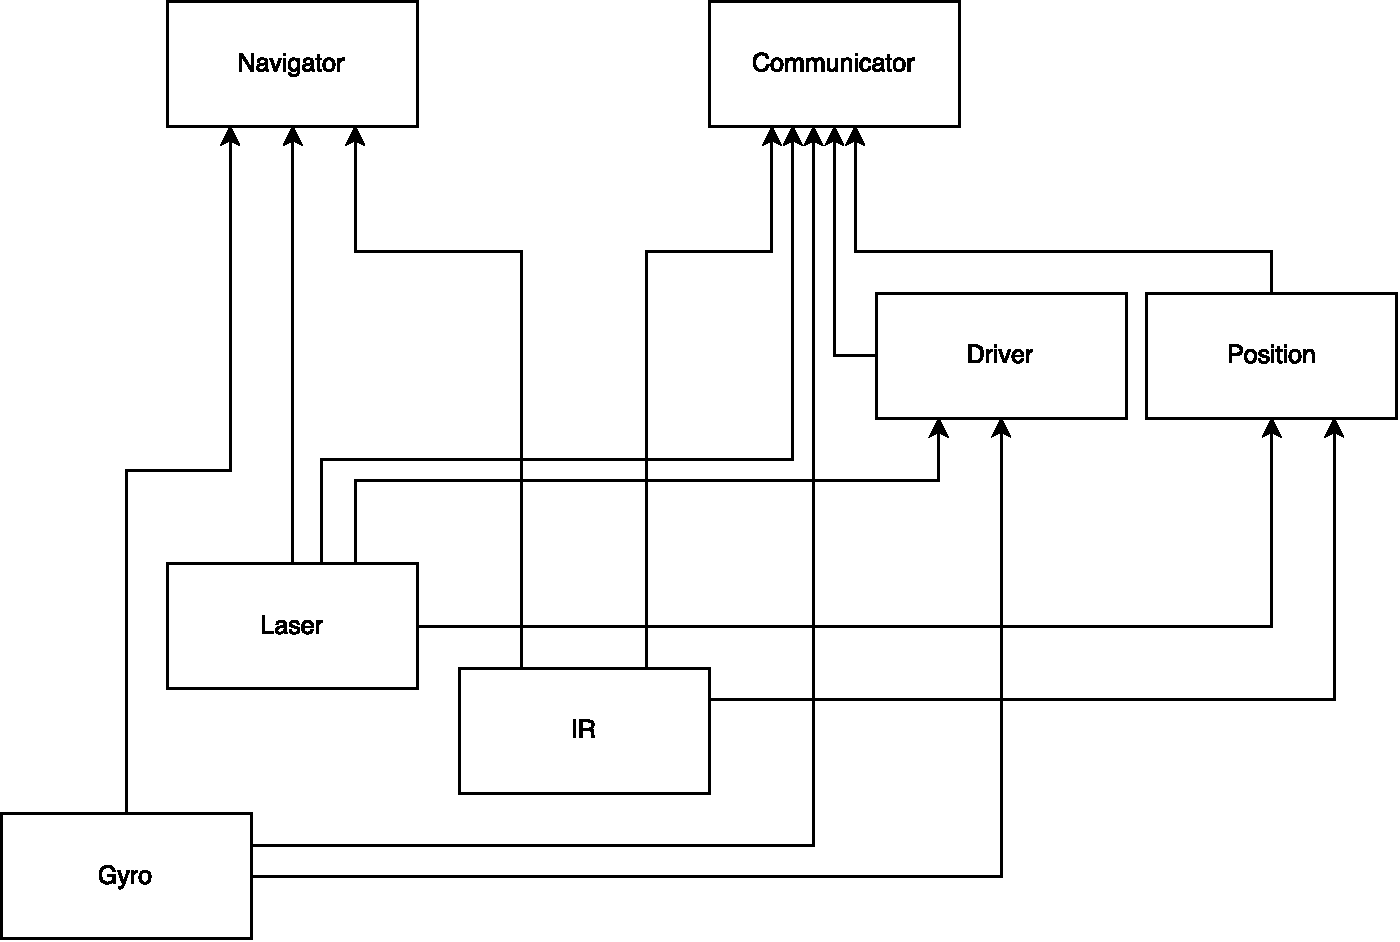
\includegraphics[scale=0.45]{mjukvarumoduler}
\caption{Ett diagram över logikenhetens mjukvarumoduler.}
\label{fig:mjukvarumoduler}
\end{figure}

\paragraph{Navigator}
Navigator-klassen sköter all logik för förflyttning. Givet viss indata från sensorerna fattar den beslut för att klarar av uppdraget. Se ~\ref{sec:navigering} för en beskrivning av navigeringsalgoritmen som används.

\paragraph{Communicator}
Communicator tar emot begäran från mjukvarumodulen och innehåller all logik för att leverera korrekt svar.
TODO:Team Bluetooth kanske vill knyta an det här till det de skriver om Bluetooth

\paragraph{Position}
\paragraph{Driver}
\paragraph{IR}
\paragraph{Laser}
\paragraph{Gyro}


\subsubsection{Kopplingsschema}

\begin{figure}[H]
\centering
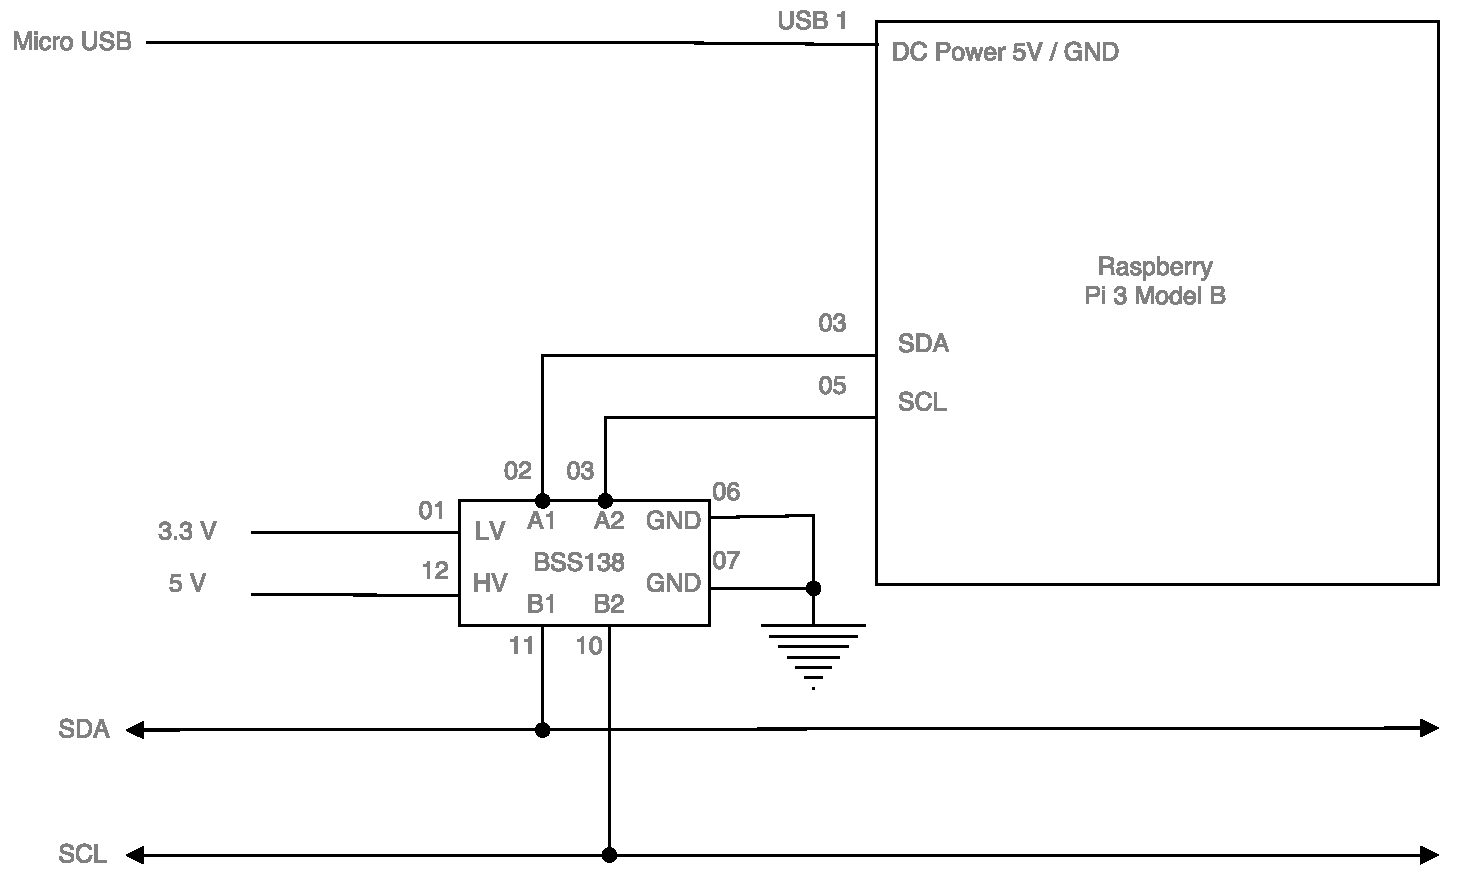
\includegraphics[scale=0.45]{Huvudenhet_kopplingsschema}
\caption{Kopplingsschema för huvudenheten.}
\label{fig:huvudenhet_kopplingsschema}
\end{figure}

Huvudenheten består av en Raspberry Pi 3 och en LCD-display av modellen JM162A. Utöver kopplingen till LCD:n så kopplas två pins till I2C-bussen. Eftersom Raspberry Pi drivs av 3.3 V matspänning och de övriga atmega-processorerna i roboten drivs av 5 V så behövs vi nivåskifta bussen så att de kan kommunicera med varandra, vilket görs med nivåskiftaren BSS138.

\subsubsection{Komponenter}

\begin{table}[H]
   \centering
  \begin{tabular}{ | c | c | }
    \hline
    \textbf{Komponent} & \textbf{Antal} \\
    \hline
    Raspberry PI 3 & 1 \\
    \hline
    JM162A & 1 \\
    \hline
  \end{tabular}
\end{table}

\subsubsection{Resurser}

\begin{table}[H]
   \centering
  \begin{tabular}{ | c | c | c | }
    \hline
    \textbf{Port} & \textbf{Antal} & \textbf{Används} \\
    \hline
    GPIO pins & 40 & 12 \\
    \hline
  \end{tabular}
\end{table}

\subsection{Sensorenhet}
Sensorenheten har i uppgift att läsa in värden från robotens sensorer och rapportera värdena till huvudenheten. Den består av fyra IR-sensorer, ett gyroskop, en lasersensor och har sin egna beräkningsenhet, en ATMega 1284, vilket låter den arbeta asynkront från andra enheter. 
\newline\newline
Den ser på så sätt alltid till att ha data tillgänglig närhelst huvudenheten begär den. För IR-sensorerna sker det genom att processorn låter AD-omvandlaren köras för en sensor i taget och sparar sedan undan avståndet i minnet, medan gyroskop och laser håller koll på sina egna värden och är kopplade direkt på I2C-bussen. Huvudenheten kan sedan fråga sensorenheten efter ny IR-mätdata, eller fråga gyroskopet/lasern direkt varpå den får sensordatan levererad över I2C.
\newline\newline
Avläsningarna från IR-sensorerna är analoga, och konverteras till digitalt med hjälp av ATMegans interna AD-omvandlare. För att sedan omvandla mätdatan till en approximation i millimeter används en tabell sparad i ATMegans minne.


\subsubsection{Kopplingsschema}
\begin{figure}[H]
\centering
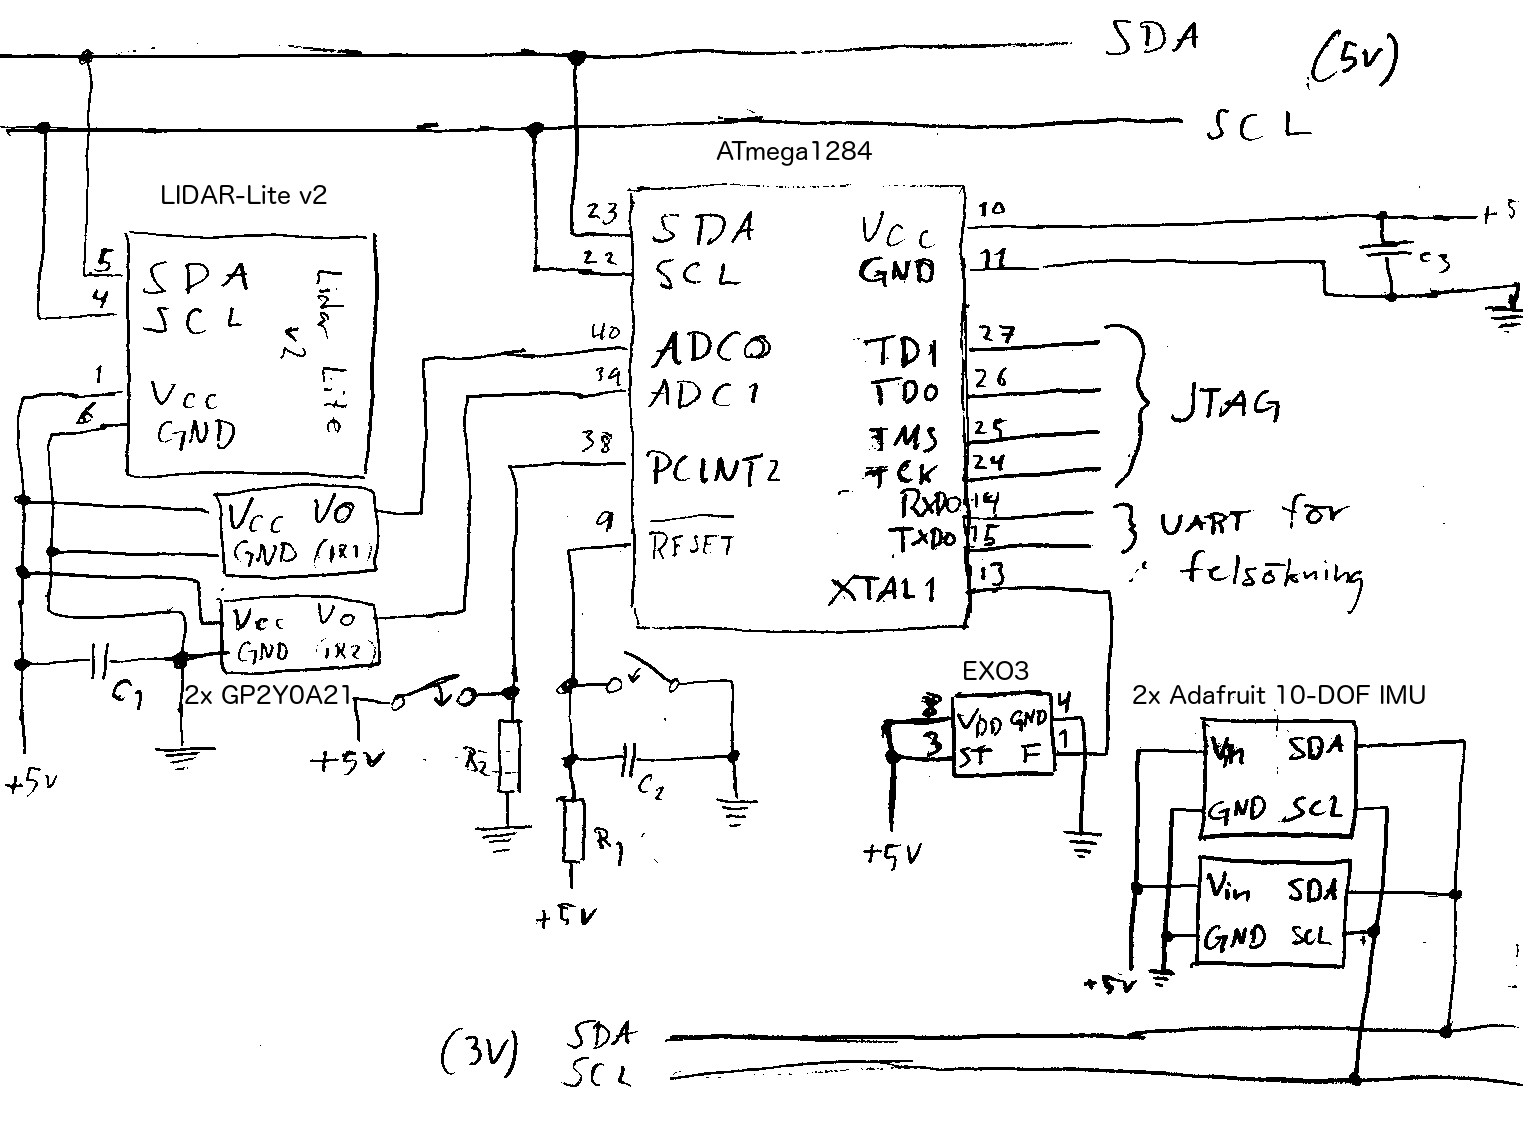
\includegraphics[scale=0.45]{Sensorenhet_kopplingsschema}
\caption{Kopplingsschema för sensorenheten.}
\label{fig:sensorenhet_kopplingsschema}
\end{figure}

Som ses i figur~\ref{fig:sensorenhet_kopplingsschema} är IR-sensorerna kopplade till ATMegan via var sitt lågpassfilter för att reducera brus. Längst upp i kopplingsschemat ses den gemensamma I2C-bussen, dit gyroskop och laser är anslutna. Notera att EXO3-komponenten är delad mellan sensorenheten och styrenheten trots att den illustreras som separata komponenter i kopplingsschemat.

\subsubsection{Komponenter}

\begin{table}[H]
  \centering
  \begin{tabular}{ | c | c | c | c |}
    \hline
    \textbf{Komponent} & \textbf{Antal} \\
    \hline
    ATMega 1284 & 1 \\
    \hline
    LIDAR-Lite v2 & 1 \\
    \hline
    Knapp & 1 \\
    \hline
    GP2Y0A41SK IR-Sensor & 3 \\
    \hline
    GP2Y0A21 IR-Sensor & 1 \\
    \hline
    Adafruit 10-DOF IMU & 1 \\
    \hline
    EXO3 & 1 (delad) \\
    \hline
  \end{tabular}
  \caption{ Tabell över de komponenter som sensorenheten består av. }
\end{table}

\subsubsection{Resurser}
% Rada upp tillgängliga portar på mikroprocessorn samt hur många som krävs
% Motivera val av mikroprocessor med uppskattning av de resurser som krävs (prestanda, minne, IO)

TODO:TABELLEN NEDAN EJ KORRIGERAD
\begin{table}[H]
  \centering
  \begin{tabular}{ | c | c | c | c |}
    \hline
    \textbf{Port} & \textbf{Antal} & \textbf{Krävs} \\
    \hline
    SDA & 1 & 1 \\
    \hline
    SCL & 1 & 1 \\
    \hline
    PCINT & 24 & 1 \\
    \hline
    A/D & 8 & 2 \\
    \hline
    RESET & 1 & 1 \\
    \hline
    USART & 4 & 2 \\
    \hline
    JTAG & 1 & 1 \\
    \hline
    CLK & 1 & 1 \\
    \hline
  \end{tabular}
  \caption{Tabell över tillgängliga portar på processorn.}
\end{table}

Den maximala hastigheten som sensordata kan läsas in i är begränsad av sensorernas rapporteringsfrekvens som är betydligt långsammare än en ATmega 1284:s klockfrekvens, därför lönar det sig inte med en snabbare processor för sensorenhetens syfte. Det i princip enda minnet sensorenheten använder sig av är för temporärlagring av alla IR-sensorers data, vilket endast motsvarar fyra heltal. Utöver sensorinläsningen kommer enheten svara på kommandon över huvudbussen som inte heller kräver några höga hastigheter eller minneskrav.

\subsubsection{Programflöde}

\begin{figure}[H]
\centering
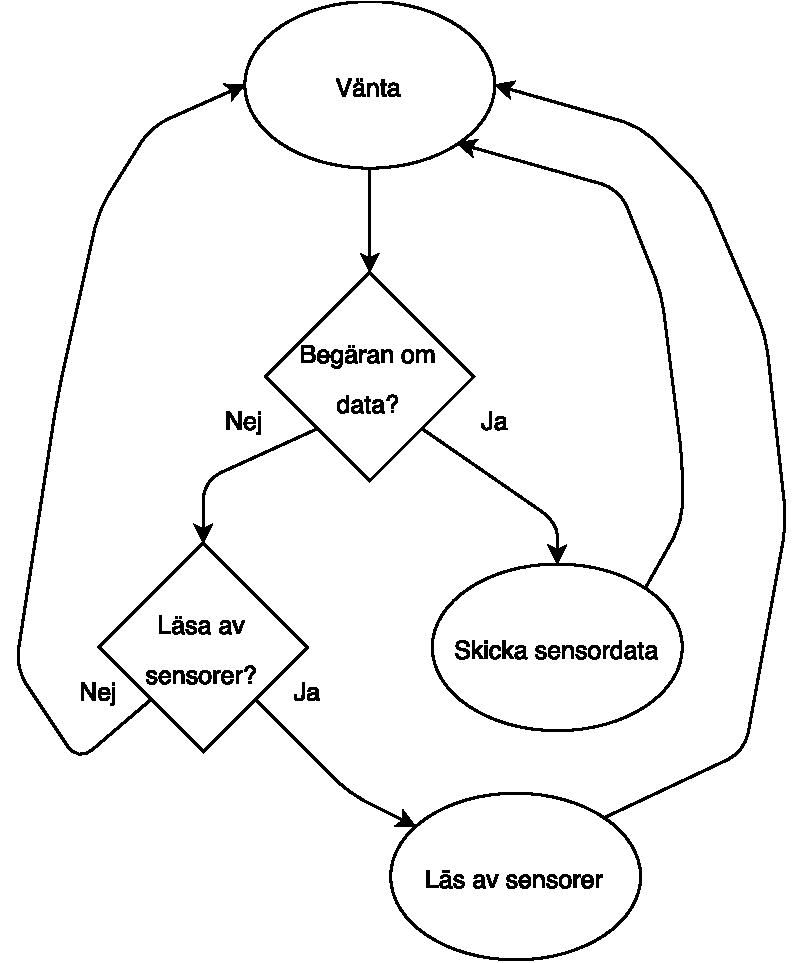
\includegraphics[scale=0.6]{sensorenhet_flowchart}
\caption{Ett flödesdiagram över sensorenhetens tillstånd}
\label{fig:sensorenhet_flowchart}
\end{figure}

För att kunna tillhandahålla sensordata från IR-sensorerna när huvudenheten ber den om det så läser sensorenheten in data med jämna mellanrum och sparar den lokalt för att sedan skicka datan på kommando från huvudenheten. Om den fått en begerän om sensordata från huvudenheten så tar det prioritet att leverera den över att läsa in ny data. Ett flödesdiagram över dess beteende ses i ~\ref{fig:sensorenhet_flowchart}.

\subsection{Styrenhet}
Styrenhetens uppgift är att kontrollera robotens förflyttning genom att ge korrekta signaler till dess hjulservon. Hjulen styrs parvis, det vill säga vänster hjulpar styrs med en signal och höger hjulpar med en annan. Hastigheten på hjulen styrs genom PWM (se avsnitt~\ref{sec:PWM}) medan hastigheter internt är definerade som heltal. Det är styrenhetens uppgift att översätta heltalshastigheter till korrekt pulskvot.

\subsubsection{Kopplingsschema}
\begin{figure}[H]
\centering
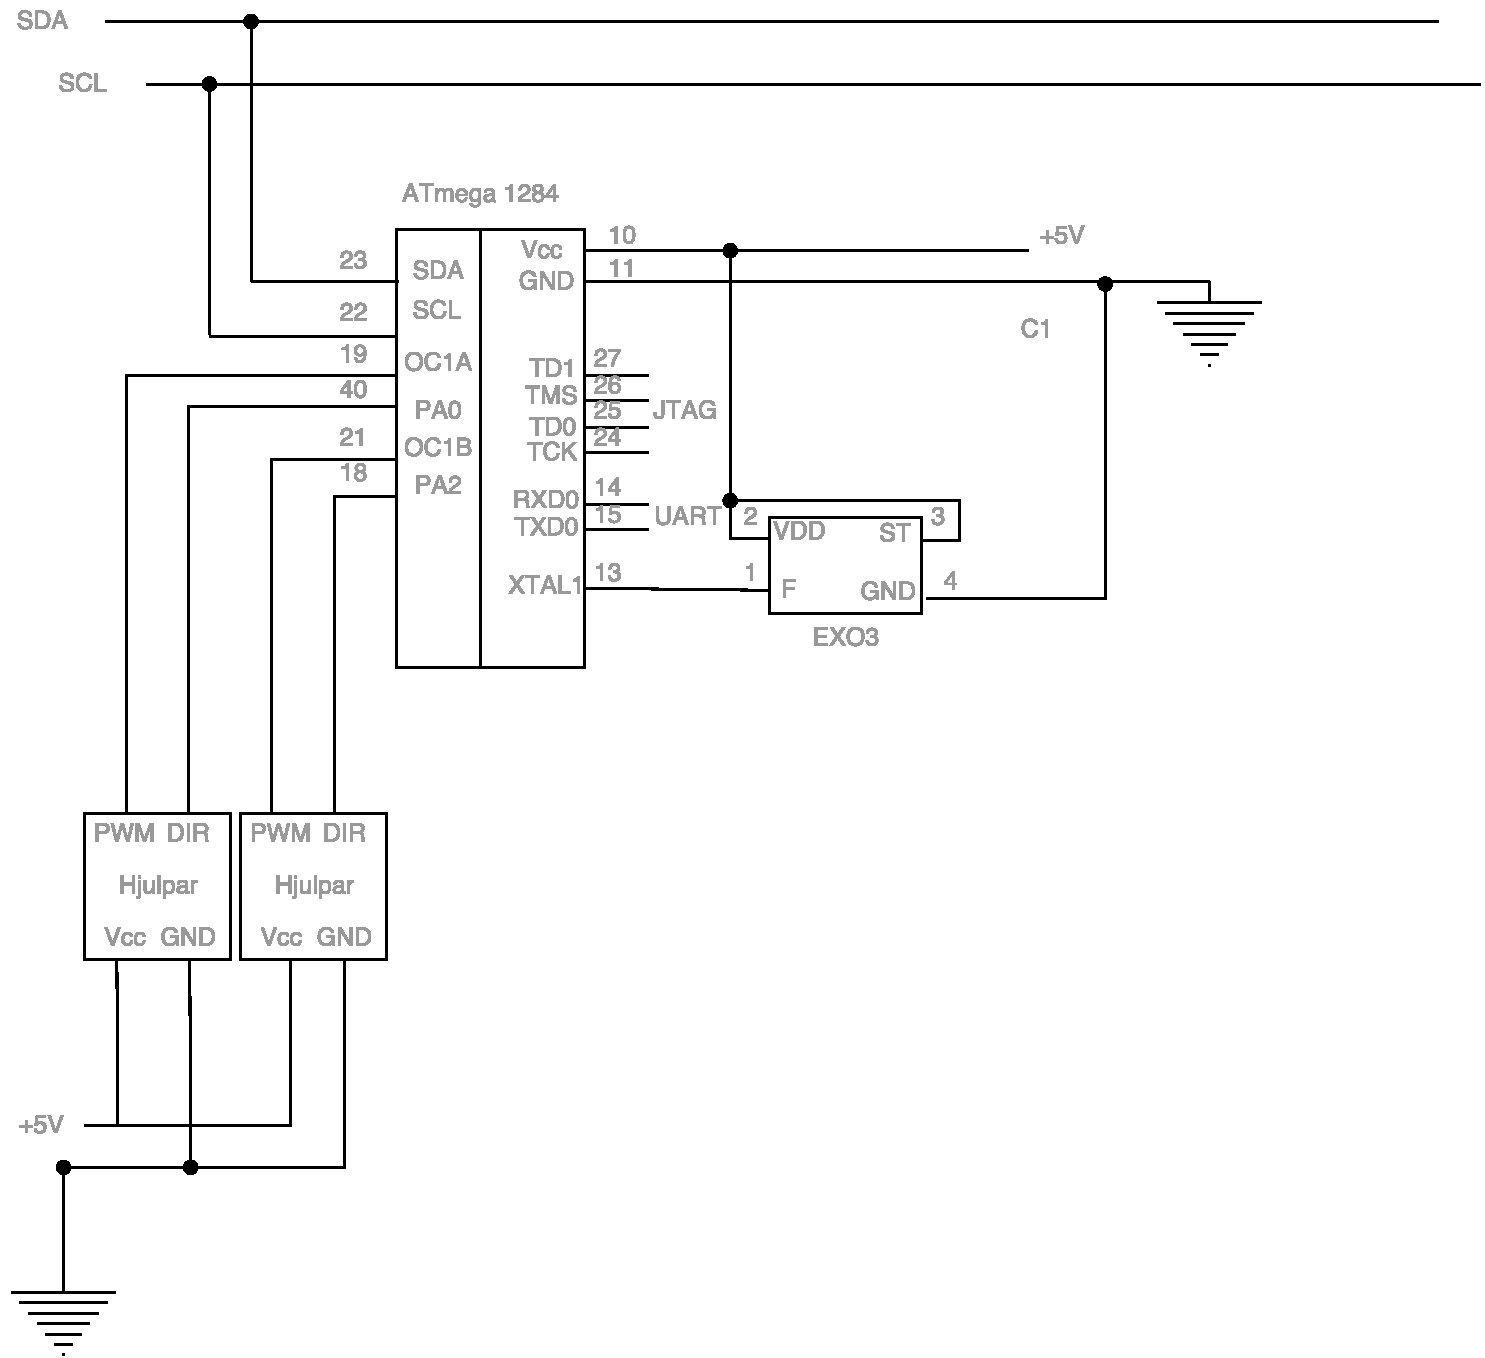
\includegraphics[scale=0.45]{Styrenhet_kopplingsschema}
\caption{Kopplingsschema för styrenheten.}
\label{fig:styrenhet_kopplingsschema}
\end{figure}



\subsubsection{Komponenter}

\begin{table}[H]
  \centering
  \begin{tabular}{ | c | c |}
    \hline
    \textbf{Komponent} & \textbf{Antal} \\
    \hline
    ATMega 1284 & 1 \\
    \hline
    Terminator (bas för fyrhjulingsrobot) & 1 \\
    \hline
    EXO3 & 1 (delad) \\
    \hline
    LS241 & 1 \\
    \hline
  \end{tabular}
\end{table}


\subsubsection{Resurser}
TODO:TABELL NEDAN EJ KORRIGERAD
\begin{table}[H]
  \centering
  \begin{tabular}{ | c | c | c | c |}
    \hline
    \textbf{Port} & \textbf{Antal} & \textbf{Krävs} \\
    \hline
    SDA & 1 & 1 \\
    \hline
    SCL & 1 & 1 \\
    \hline
    RESET & 1 & 1 \\
    \hline
    IO & 30 & 5 \\
    \hline
    USART & 4 & 4 \\
    \hline
    JTAG & 1 & 1 \\
    \hline
    CLK & 1 & 1 \\
    \hline
  \end{tabular}
  \caption{Tabell över tillgängliga portar på processorn.}
\end{table}

Omvandlingen av kommandon från huvudenheten och utskickning av signaler till servona uppskattas ej kräva mer prestanda eller minne än styrenhetens ATMega 1284 processor klarar av.

\subsubsection{Programflöde}

\begin{figure}[H]
\centering
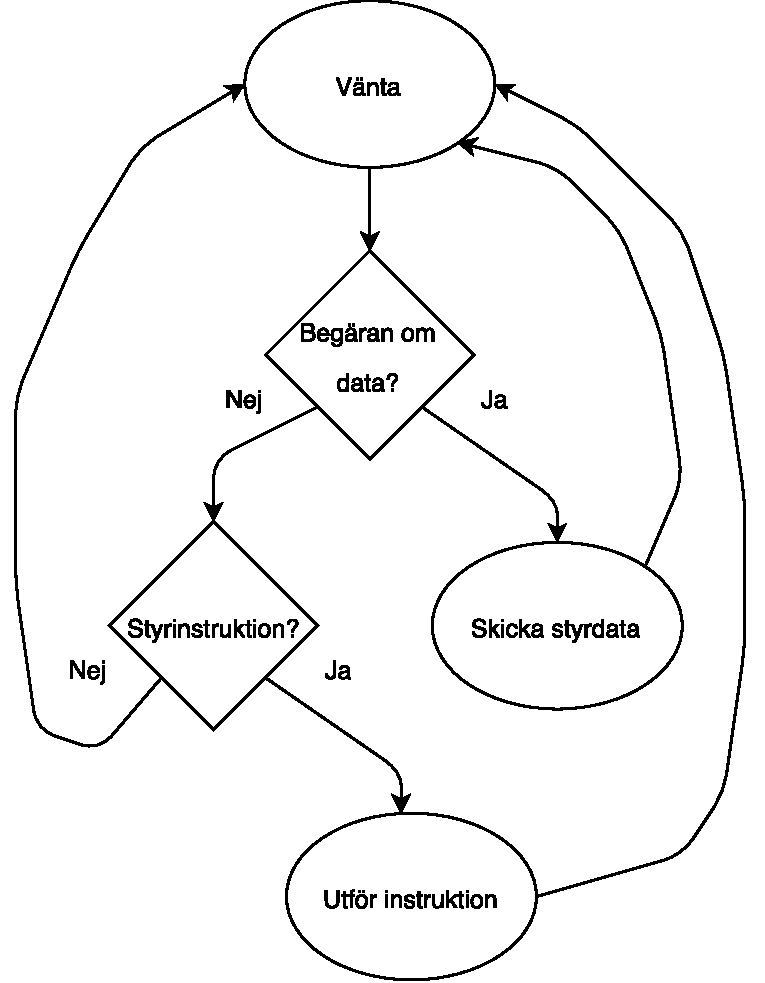
\includegraphics[scale=0.6]{styrenhet_flowchart}
\caption{Ett flödesschema över styrenhetens tillstånd}
\label{fig:styrenhet_flowchart}
\end{figure}

Styrenheten står hela tiden och väntar på instruktioner från huvudenheten, och så snart den får några utför den dem så snabbt den kan. En instruktion i det här sammamhanget är att sätta nya hastigheter på de båda hjulparen. Ett flödesschema över styrenhetens beteende kan ses i figur ~\ref{fig:styrenhet_flowchart}.

\clearpage
\section{Slutsatser}
% Vilka förbättringar skulle kunna göras?

\subsection{Navigeringsalgoritm}
\label{sec:slutsatser_navigering}
Vår navigeringsalgoritm är i nuläget begränsad till att röra sig i ett rutnät och får således bara röra sig i vinklar som är multiplar av 90 grader. Begränsningen beror på att roboten inte har någon bra logik för att bestämma sin position utan att följa en vägg. Om roboten skulle kunna bestämma sin position när den navigerade i godtycklig riktning och på öppna ytor hade den totala sträckan som roboten behövt färdas minimeras.

\subsection{Kartläggning}
Roboten kartläggningsalgoritm kartlägger sin omgivning genom att beräkna raksträckor den åkt när den följt en vägg och spara start- och slut-koordinaterna. Om roboten kunde observera sin omgivning t.ex. med en svepande laser och beräkna var väggar fanns utifrån den datan så skulle den ej behöva färdas längs med alla väggar för att kartlägga dem. Det här förbättringsförslaget går hand i hand med förbättringarna föreslagna i avsnitt ~\ref{sec:slutsatser_navigering}.

\clearpage
\section{Referenser}
\appendix
%Appendix
%A. Kopplingsschema
%B. Programlistning och eventuell VHDL kod
%C. Övrigt (typ banspec)
\clearpage
\section{Banspecifikation}
\label{sec:banspec}

\clearpage
\section{Programkod}

\end{document}
